\section{Resultados preliminares de las mediciones recibidas}
\label{sec:resultados}

Se procesaron los cuatro CSV de latencia publicados el 19 de noviembre
de 2026. Contienen 4\,000 filas: 1\,600 de sockets y 2\,400 de gRPC.
De gRPC se excluyeron 800 filas marcadas como calentamiento.
El análisis utiliza 3\,200 mensajes válidos, agrupados por mecanismo,
equipo, modo y tamaño. Las tablas se leen directamente de las salidas
de \texttt{analysis/analizar.py}.

Los registros de sockets tienen un formato de seis columnas. El lector
los adapta en memoria y utiliza el nodo y el número de envío para
identificar cada mensaje dentro de su corrida. El modo se indica por
argumento. El equipo aparece como \texttt{sin-registrar} porque ese dato
falta en los CSV y en la descripción del entorno de sockets.

\begin{table}[htbp]
\centering
\small
\caption{Mediciones experimentales. Latencias en milisegundos; desviación estándar muestral por mensaje.}
\resizebox{\linewidth}{!}{%
\begin{tabular}{llllrrrr}
\toprule
Equipo & Modo & Bytes & Mecanismo & Media & Mediana & Desv. & P95 \\
\midrule
DESKTOP-5MJCPHU & concurrente & 100 & grpc & 0.4980 & 0.4771 & 0.0960 & 0.7042 \\
DESKTOP-5MJCPHU & concurrente & 10000 & grpc & 0.5557 & 0.5455 & 0.0992 & 0.7308 \\
DESKTOP-5MJCPHU & secuencial & 100 & grpc & 0.2929 & 0.2772 & 0.0709 & 0.3823 \\
DESKTOP-5MJCPHU & secuencial & 10000 & grpc & 0.3306 & 0.3057 & 0.0885 & 0.4746 \\
sin-registrar & concurrente & 100 & sockets & 0.0909 & 0.0787 & 0.0662 & 0.1512 \\
sin-registrar & concurrente & 10000 & sockets & 0.1458 & 0.1364 & 0.0524 & 0.2083 \\
sin-registrar & secuencial & 100 & sockets & 0.0520 & 0.0470 & 0.0207 & 0.0682 \\
sin-registrar & secuencial & 10000 & sockets & 0.0762 & 0.0704 & 0.0218 & 0.0924 \\
\bottomrule
\end{tabular}
}
\end{table}

\begin{table}[htbp]
\centering
\small
\caption{Mediciones experimentales. Rendimiento agregado: mensajes completados / tiempo total de corridas.}
\resizebox{\linewidth}{!}{%
\begin{tabular}{llllrrrr}
\toprule
Equipo & Modo & Bytes & Mecanismo & Mensajes & Corridas & Tiempo (s) & Mensajes/s \\
\midrule
DESKTOP-5MJCPHU & concurrente & 100 & grpc & 300 & 1 & 0.2189 & 1370.3448 \\
DESKTOP-5MJCPHU & concurrente & 10000 & grpc & 300 & 1 & 0.2184 & 1373.4817 \\
DESKTOP-5MJCPHU & secuencial & 100 & grpc & 500 & 5 & 1.0718 & 466.5115 \\
DESKTOP-5MJCPHU & secuencial & 10000 & grpc & 500 & 5 & 1.0600 & 471.7035 \\
sin-registrar & concurrente & 100 & sockets & 300 & 1 & N/D & N/D \\
sin-registrar & concurrente & 10000 & sockets & 300 & 1 & N/D & N/D \\
sin-registrar & secuencial & 100 & sockets & 500 & 5 & N/D & N/D \\
sin-registrar & secuencial & 10000 & sockets & 500 & 5 & N/D & N/D \\
\bottomrule
\end{tabular}
}
\end{table}


Ambos mecanismos tienen cinco corridas secuenciales de 100 envíos por
tamaño y una corrida concurrente de 300 mensajes por tamaño.
Los registros gRPC identifican el equipo \texttt{DESKTOP-5MJCPHU}.
Falta documentar el equipo de sockets y ejecutar ambos mecanismos
bajo condiciones equivalentes en cada máquina. Estas observaciones
permiten describir las sesiones recibidas; una conclusión sobre la
hipótesis requiere controlar esas diferencias de entorno.

\subsection{Duración y límites de medición}
Los CSV de sockets carecen de duración total de corrida. Por ello,
su tiempo total y rendimiento quedan como N/D en las salidas.
Las tasas de gRPC se calculan a partir de la duración registrada por
su programa, cuyo intervalo incluye la preparación o espera de los
canales además de los envíos. El alcance de ese intervalo deberá
mantenerse equivalente cuando se mida sockets.

Los tamaños declarados en ambos programas son 100 y 10\,000 bytes
de solicitud serializada. En sockets se ajusta el JSON con el salto de
línea; en gRPC se usa \texttt{ByteSize()} de Protocol Buffers.
La serialización JSON se realiza antes del cronómetro, mientras que
la llamada gRPC medida incorpora su serialización interna. Esta
diferencia debe considerarse al interpretar las latencias.

\begin{figure}[p]
\centering
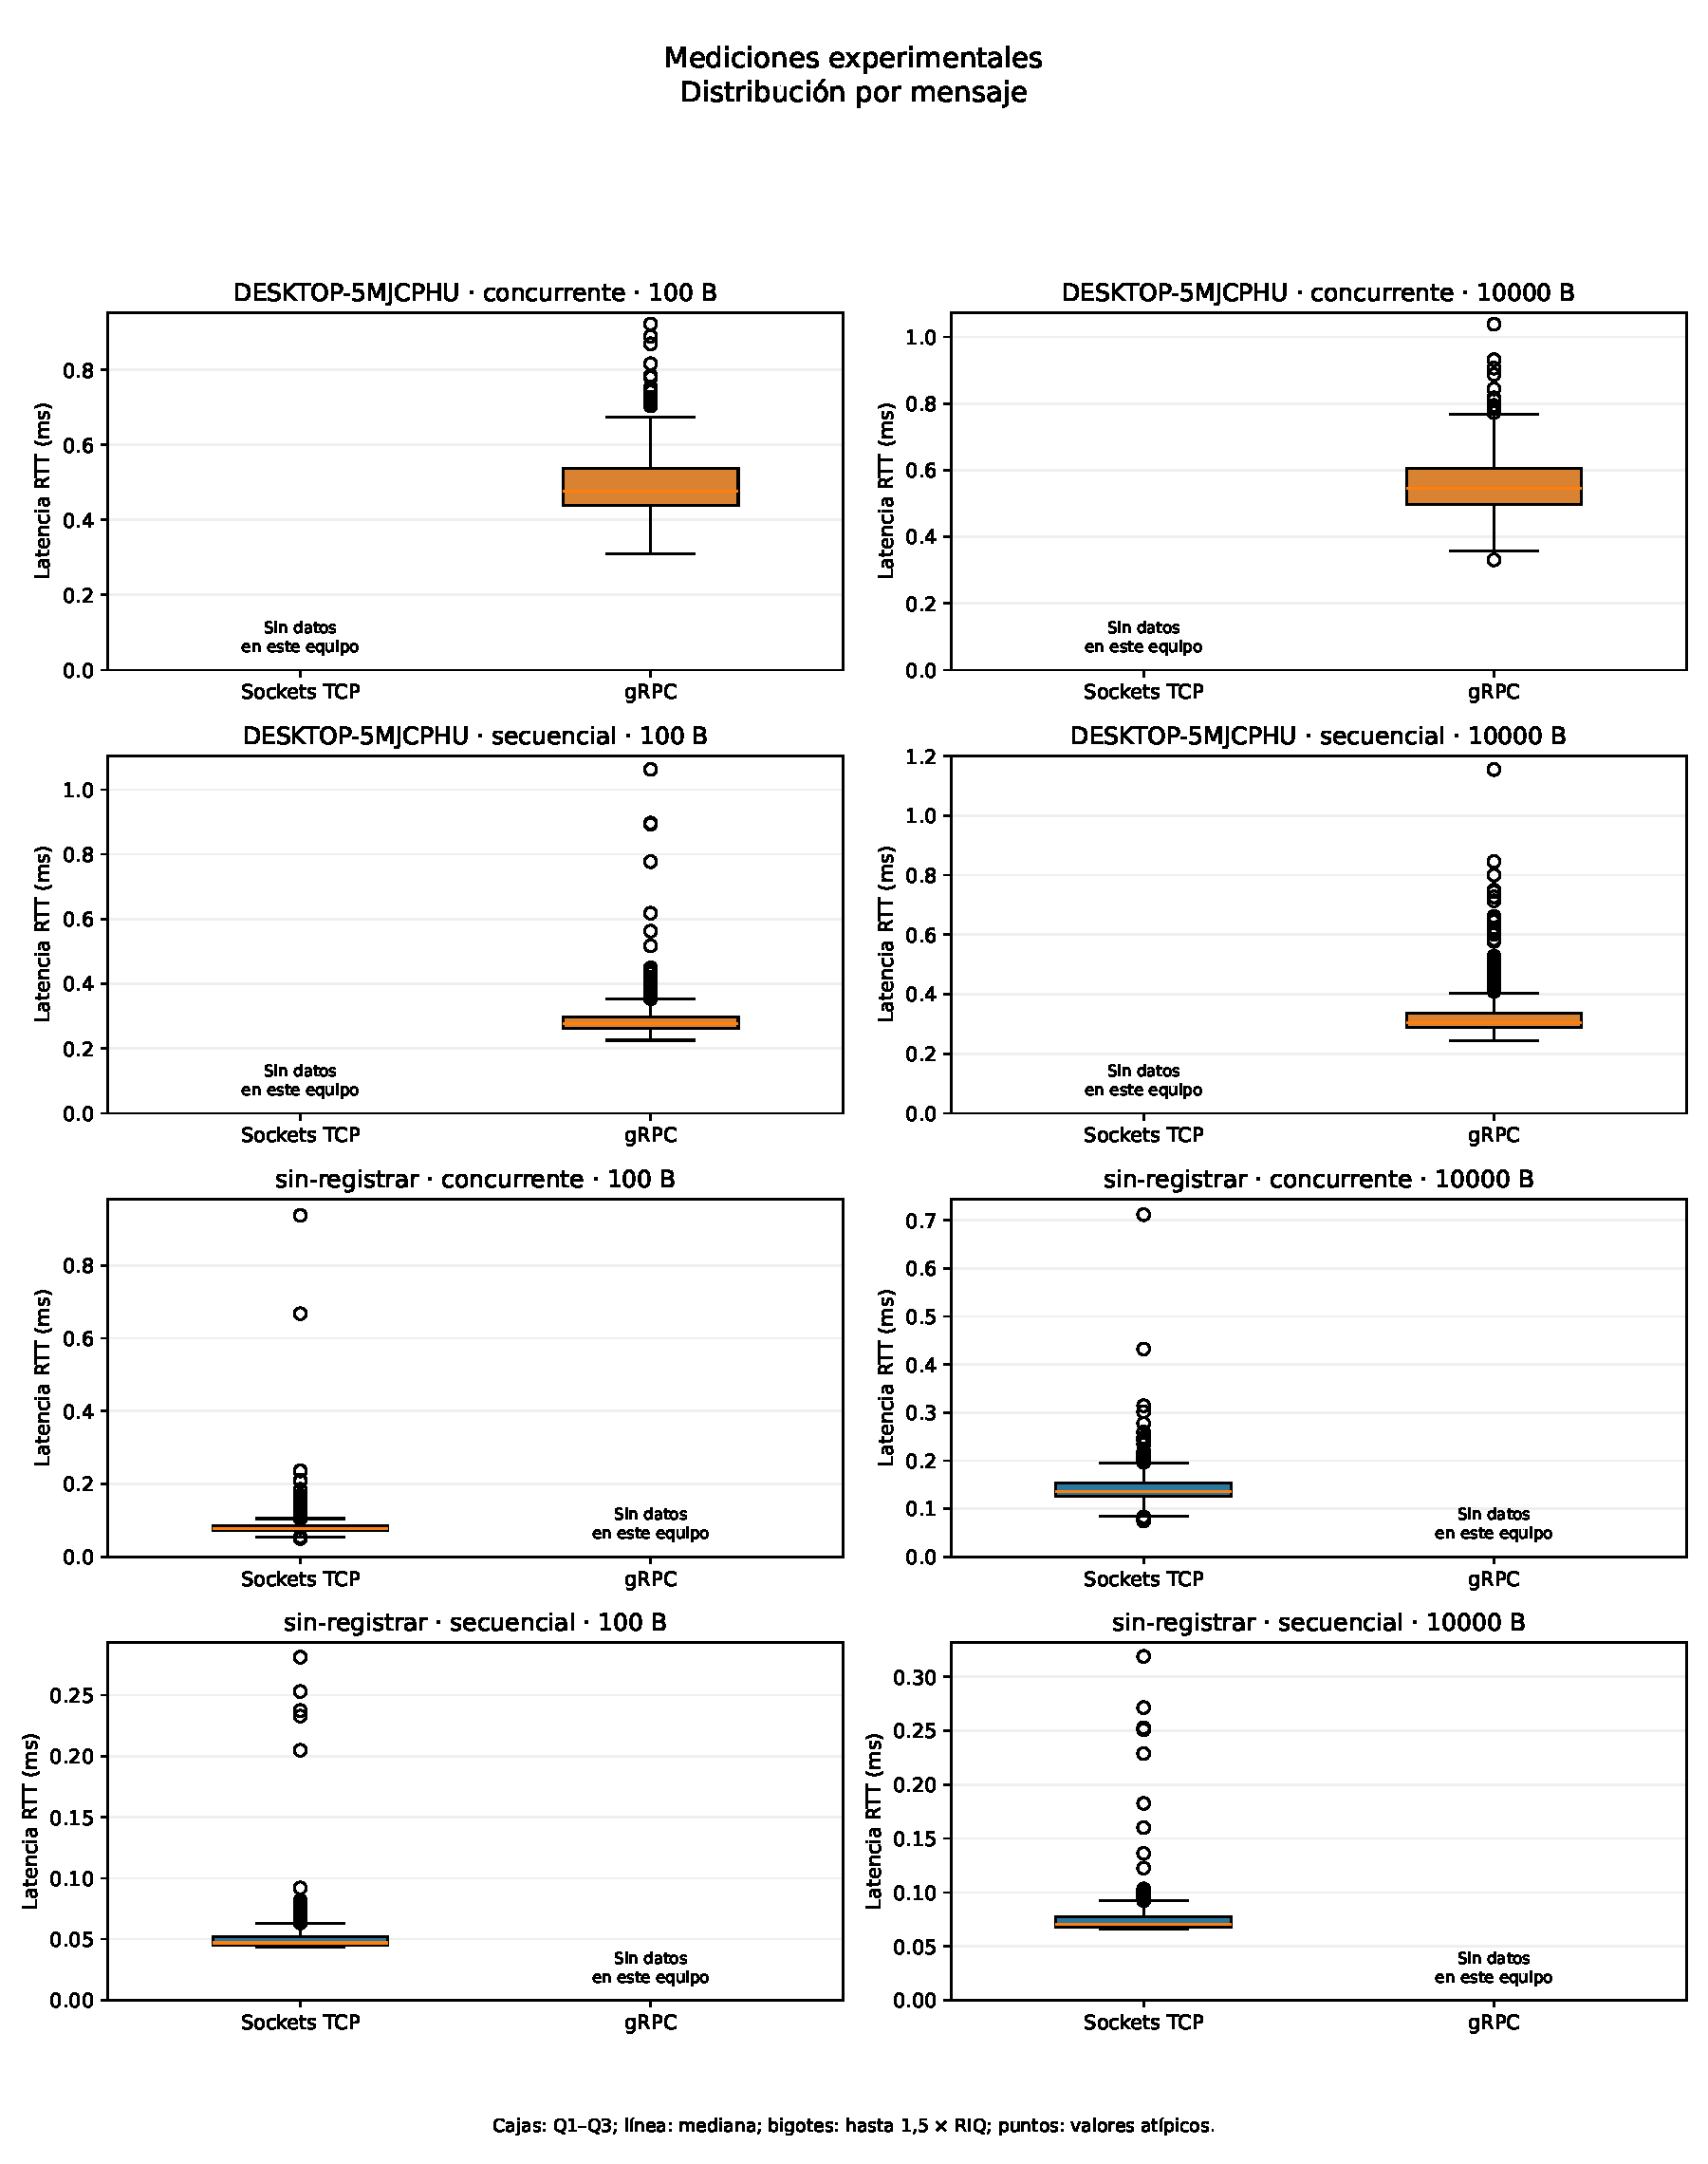
\includegraphics[width=\linewidth,height=0.83\textheight,keepaspectratio]{../analysis/resultados-2026-11-19/cajas_latencias.pdf}
\caption{Distribución de latencias de los registros reales recibidos.
Las condiciones se separan por equipo, modo y tamaño.}
\label{fig:latencias-reales-cajas}
\end{figure}
\begin{figure}[p]
\centering
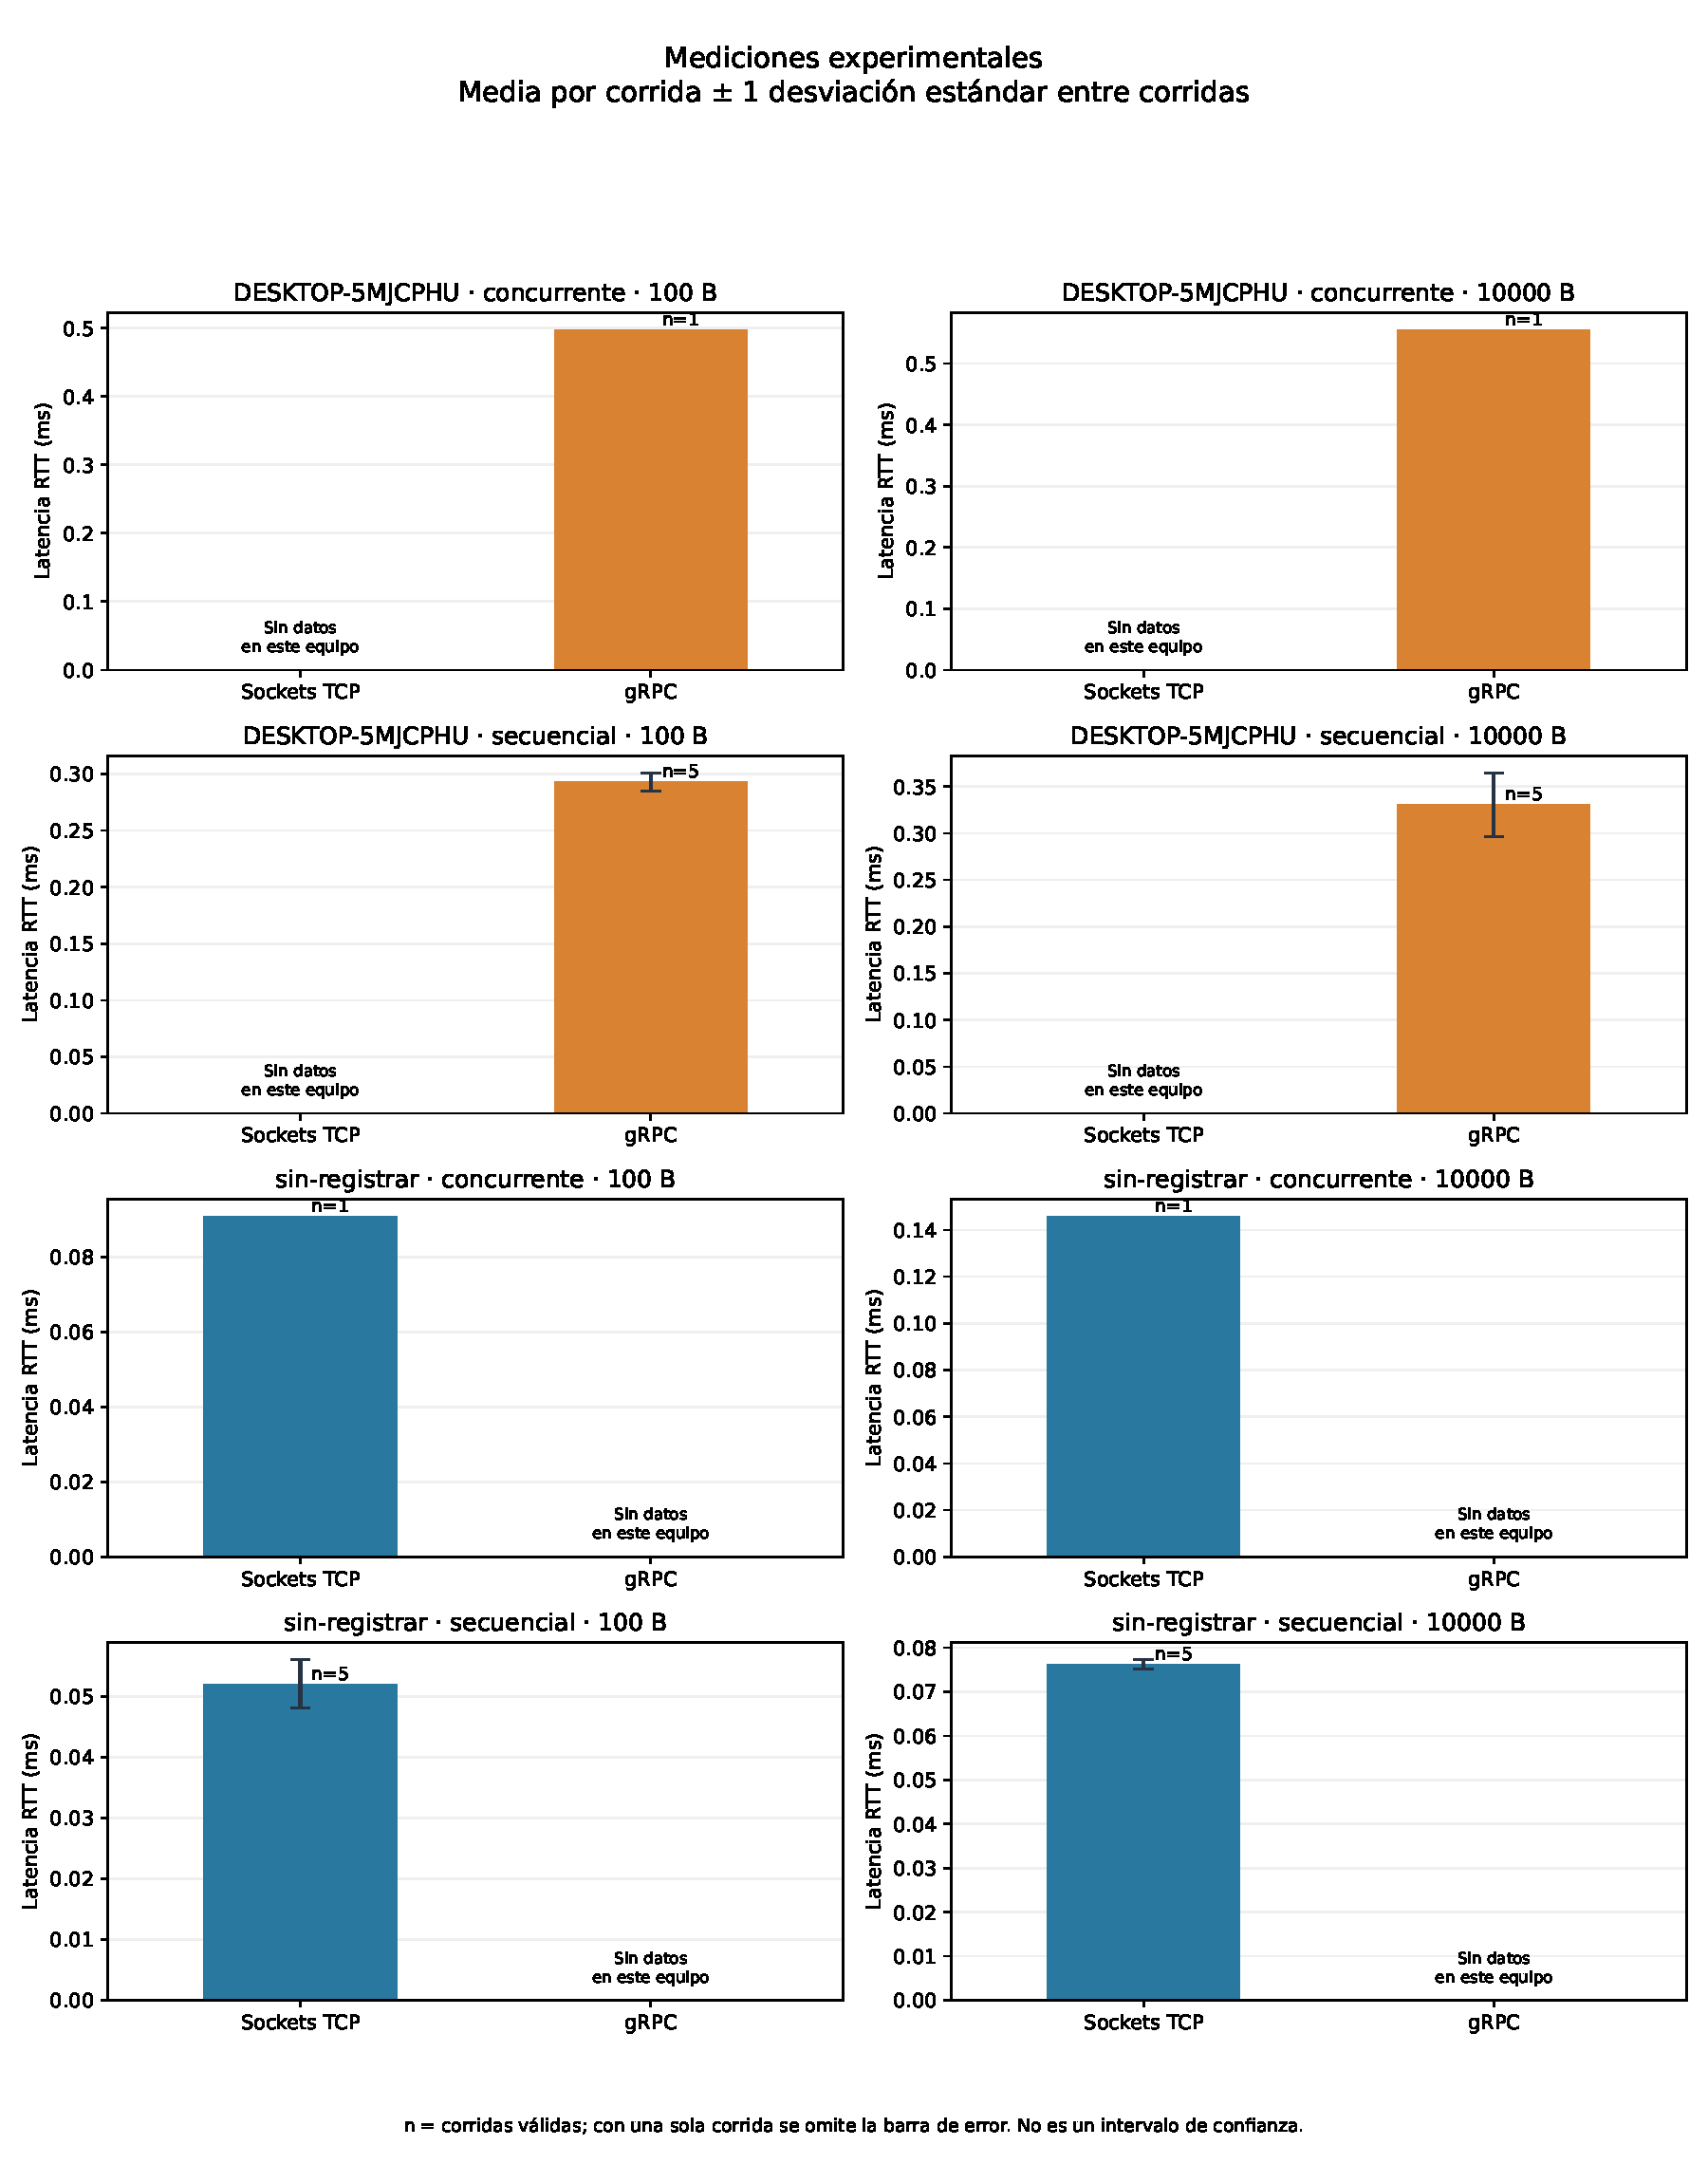
\includegraphics[width=\linewidth,height=0.83\textheight,keepaspectratio]{../analysis/resultados-2026-11-19/barras_latencias.pdf}
\caption{Medias por corrida de los registros reales recibidos.
El intervalo representa una desviación estándar entre medias.
Cada barra indica el número de repeticiones disponibles; con una
sola corrida concurrente se omite el intervalo.}
\label{fig:latencias-reales-barras}
\end{figure}
